\begin{figure*}
  \centering

\begin{subfigure}[b]{0.4\textwidth}
\centering
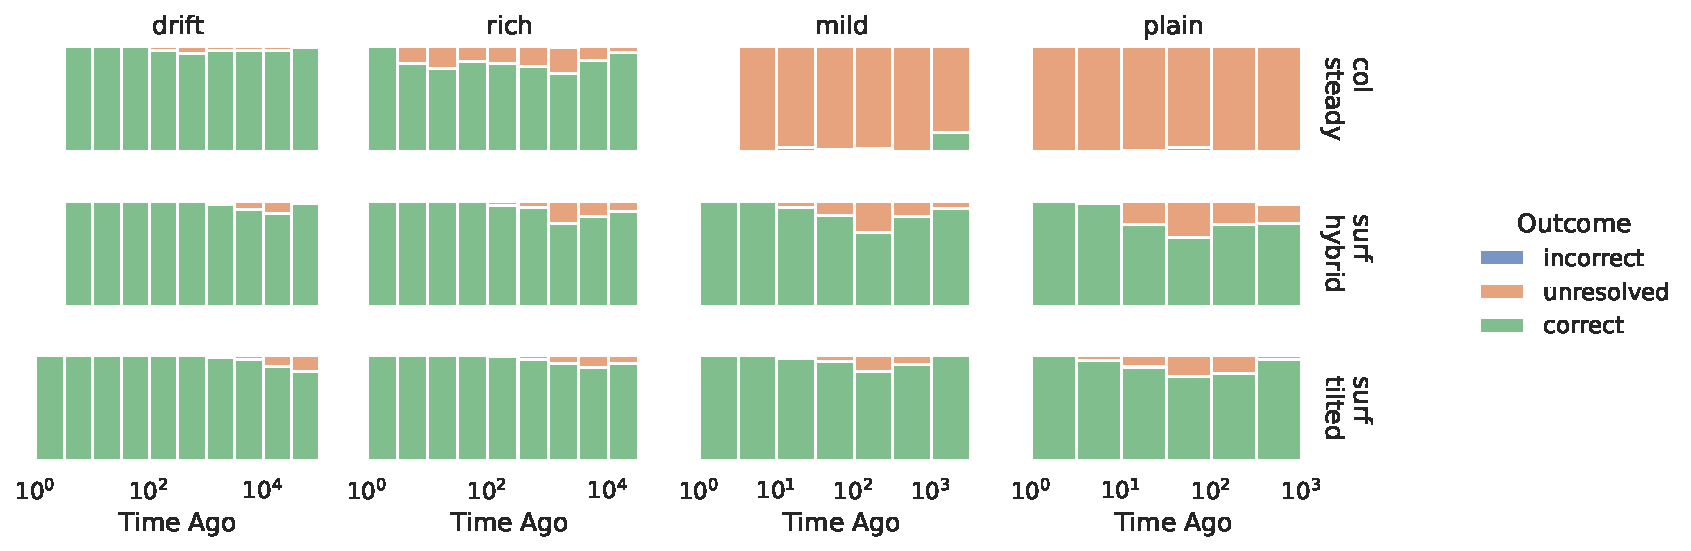
\includegraphics[height=1.2in,trim={0 0 5cm 0},clip]{binder/binder/teeplots/annotation-size-bits=256+col=scenario+differentia-width-bits=8+hue=outcome+kind=hist+multiple=fill+row=algo+scale=npop65536-ngen100000+viz=displot+x=time-ago+ext=}
\caption{256 bits, 8 bit width}
\end{subfigure}%
\begin{subfigure}[b]{0.6\textwidth}
\centering
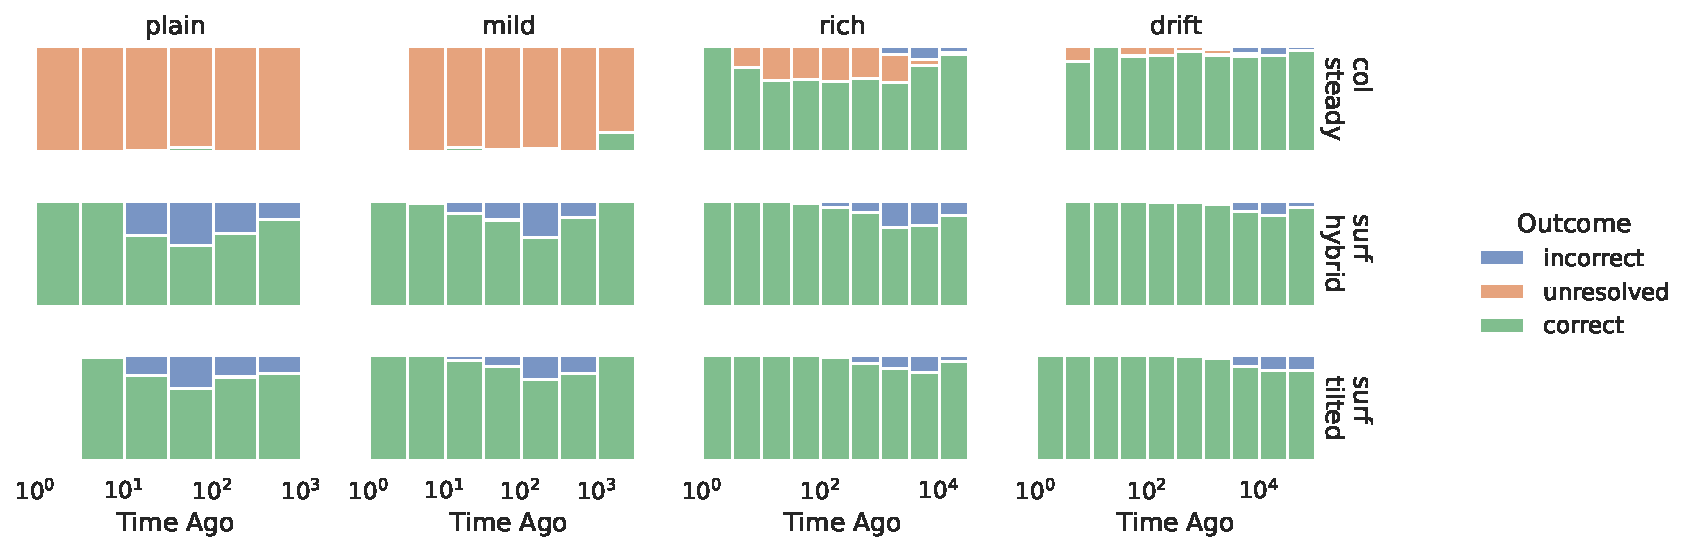
\includegraphics[height=1.2in]{binder/binder/teeplots/annotation-size-bits=32+col=scenario+differentia-width-bits=1+hue=outcome+kind=hist+multiple=fill+row=algo+scale=npop65536-ngen100000+viz=displot+x=time-ago+ext=}
\caption{32 bits, 1 bit width}
\end{subfigure}

\begin{subfigure}[b]{0.4\textwidth}
  \centering
  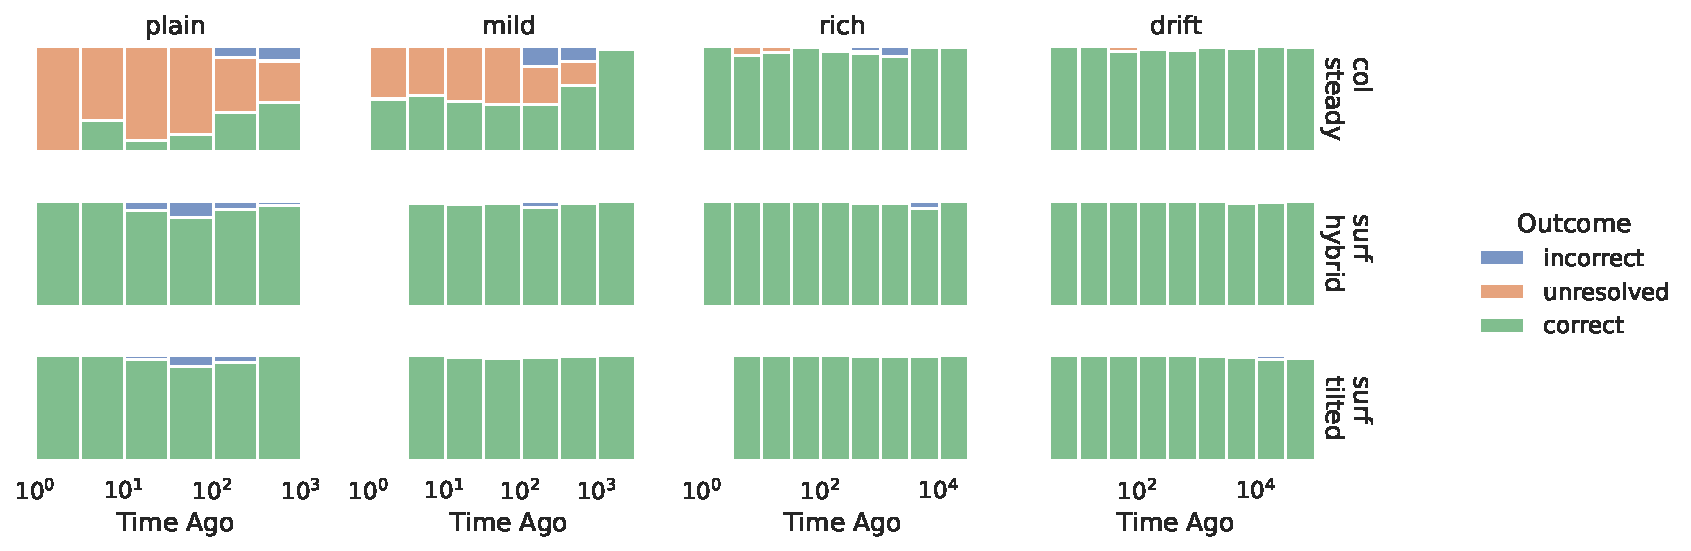
\includegraphics[height=1.2in,trim={0 0 5cm 0},clip]{binder/binder/teeplots/annotation-size-bits=256+col=scenario+differentia-width-bits=1+hue=outcome+kind=hist+multiple=fill+row=algo+scale=npop65536-ngen100000+viz=displot+x=time-ago+ext=}
  \caption{256 bits, 1 bit width}
  \end{subfigure}%
  \begin{subfigure}[b]{0.6\textwidth}
    \flushright
    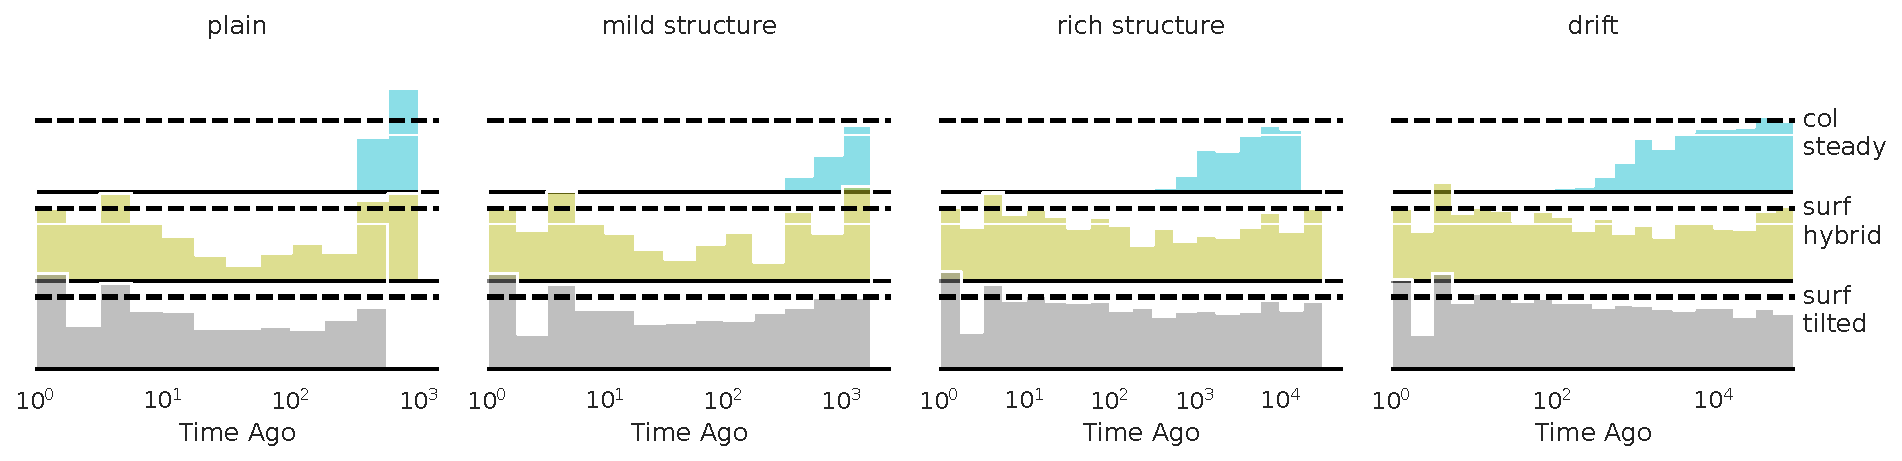
\includegraphics[height=1.2in,width=0.95\linewidth]{binder/binder/teeplots/annotation-size-bits=256+col=scenario+differentia-width-bits=8+hue=kind+row=algo+scale=npop65536-ngen100000+viz=joyhist+x=time-ago+ext=}
    \caption{TODO}
  \end{subfigure}%
  \caption{TODO}
  \label{fig:recency-structure}

\end{figure*}
